\documentclass[tikz,border=1pt]{standalone}
\usepackage{amsmath,amssymb}
\usetikzlibrary{positioning,arrows.meta,calc,fit,backgrounds}
\definecolor{cHyb}{HTML}{0072B2}
\definecolor{cProg}{HTML}{D55E00}
\definecolor{cNat}{HTML}{8C8C8C}
\definecolor{cTxt}{HTML}{404040}
\begin{document}
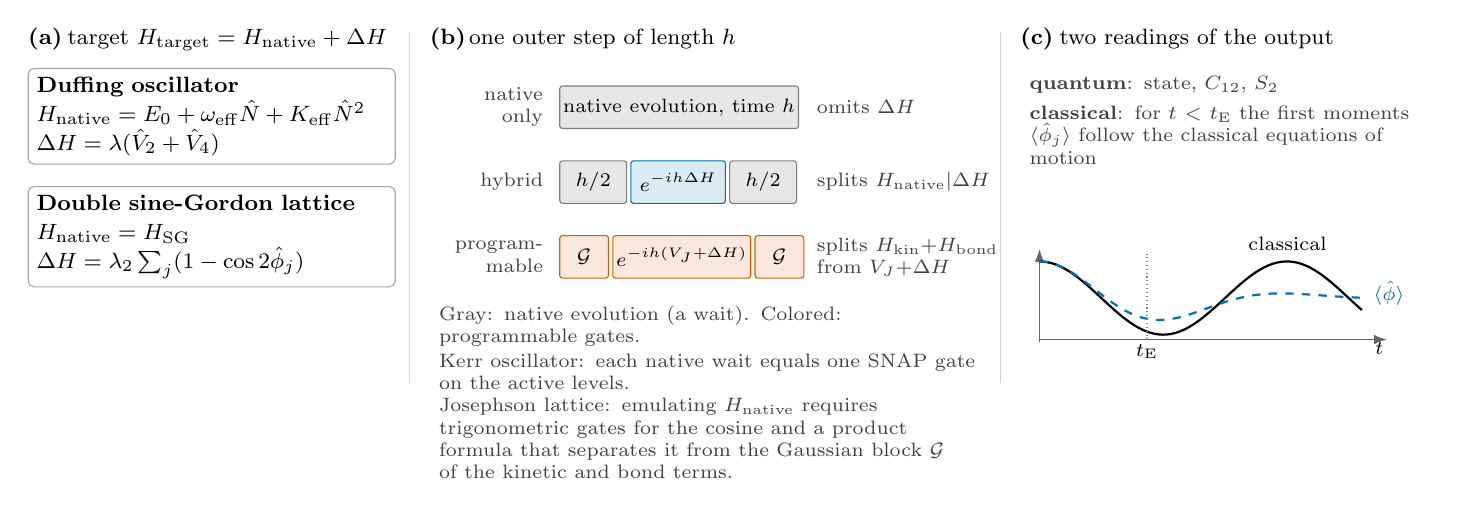
\begin{tikzpicture}[
  font=\footnotesize, >={Latex[length=1.6mm,width=1.2mm]},
  lab/.style={font=\footnotesize\bfseries, anchor=base west, inner sep=0pt},
  head/.style={font=\footnotesize, anchor=base west, inner sep=0pt},
  card/.style={draw=black!35, rounded corners=2pt, inner sep=3pt, align=left, fill=white, text width=4.45cm},
  nat/.style={draw=cNat!90!black, fill=cNat!22, minimum height=5.4mm, inner sep=1.2pt, rounded corners=1pt, font=\scriptsize},
  prog/.style={draw=cProg, fill=cProg!14, minimum height=5.4mm, inner sep=1.2pt, rounded corners=1pt, font=\scriptsize},
  hyb/.style={draw=cHyb, fill=cHyb!14, minimum height=5.4mm, inner sep=1.2pt, rounded corners=1pt, font=\scriptsize},
  rowlab/.style={font=\scriptsize, anchor=east, align=right, text=cTxt},
  note/.style={font={\scriptsize\hyphenpenalty=10000\exhyphenpenalty=10000}, text=cTxt, align=left},
]
\def\ytop{3.0}
% ---------------- (a) target
\node[lab] at (0,\ytop) {(a)};
\node[head] at (0.5,\ytop) {target $H_{\rm target}=H_{\rm native}+\Delta H$};
\node[card, anchor=north west] (duf) at (0,2.7) {%
  \textbf{Duffing oscillator}\\[1pt]
  $H_{\rm native}=E_0+\omega_{\rm eff}\hat N+K_{\rm eff}\hat N^{2}$\\[1pt]
  $\Delta H=\lambda(\hat V_{2}+\hat V_{4})$};
\node[card, anchor=north west] (dsg) at (0,1.2) {%
  \textbf{Double sine-Gordon lattice}\\[1pt]
  $H_{\rm native}=H_{\rm SG}$\\[1pt]
  $\Delta H=\lambda_2\sum_j(1-\cos 2\hat\phi_j)$};

% ---------------- (b) one step
\def\xb{5.1}
\def\xs{6.75}
\def\ya{2.2} \def\yb{1.25} \def\yc{0.3}
\node[lab] at (\xb,\ytop) {(b)};
\node[head] at (\xb+0.5,\ytop) {one outer step of length $h$};
\node[rowlab] at (\xs-0.08,\ya) {native\\only};
\node[nat, minimum width=2.98cm, anchor=west] (n1) at (\xs,\ya) {native evolution, time $h$};
\node[rowlab] at (\xs-0.08,\yb) {hybrid};
\node[nat, minimum width=0.85cm, anchor=west] (h1) at (\xs,\yb) {$h/2$};
\node[hyb, minimum width=1.2cm, anchor=west] (h2) at ($(h1.east)+(0.04,0)$) {$e^{-ih\Delta H}$};
\node[nat, minimum width=0.85cm, anchor=west] (h3) at ($(h2.east)+(0.04,0)$) {$h/2$};
\node[rowlab] at (\xs-0.08,\yc) {program-\\mable};
\node[prog, minimum width=0.62cm, anchor=west] (p1) at (\xs,\yc) {$\mathcal G$};
\node[prog, minimum width=1.66cm, anchor=west] (p2) at ($(p1.east)+(0.04,0)$) {$e^{-ih(V_J+\Delta H)}$};
\node[prog, minimum width=0.62cm, anchor=west] (p3) at ($(p2.east)+(0.04,0)$) {$\mathcal G$};
\node[note, anchor=west] at (9.9,\ya) {omits $\Delta H$};
\node[note, anchor=west] at (9.9,\yb) {splits $H_{\rm native}|\Delta H$};
\node[note, anchor=west, text width=2.35cm] at (9.9,\yc) {splits $H_{\rm kin}{+}H_{\rm bond}$ from $V_J{+}\Delta H$};
\node[note, anchor=north west, text width=6.9cm] at (\xb,-0.2) {%
  Gray: native evolution (a wait). Colored: programmable gates.\\[1pt]
  Kerr oscillator: each native wait equals one SNAP gate on the active levels.\\
  Josephson lattice: emulating $H_{\rm native}$ requires trigonometric gates for the cosine and a product formula that separates it from the Gaussian block $\mathcal G$ of the kinetic and bond terms.};

% ---------------- (c) outputs
\def\xc{12.6}
\node[lab] at (\xc,\ytop) {(c)};
\node[head] at (\xc+0.5,\ytop) {two readings of the output};
\node[note, anchor=north west, text width=4.95cm] at (\xc,2.72) {%
  \textbf{quantum}: state, $C_{12}$, $S_2$\\[3pt]
  \textbf{classical}: for $t<t_{\rm E}$ the first moments $\langle\hat\phi_j\rangle$ follow the classical equations of motion};
\begin{scope}[shift={(\xc+0.25,-0.75)}, x=1.05cm, y=0.62cm]
  \draw[->, black!60] (0,0) -- (4.2,0) node[below left, font=\scriptsize, text=black, inner sep=1pt] {$t$};
  \draw[->, black!60] (0,-0.05) -- (0,1.85);
  \draw[black, thick, domain=0:3.9, samples=90] plot (\x,{0.85+0.75*cos(deg(2.1*\x))});
  \draw[cHyb, thick, dashed, domain=0:3.9, samples=90] plot (\x,{0.85+0.75*exp(-0.22*(\x)^2)*cos(deg(1.95*\x))});
  \draw[black!50, densely dotted] (1.3,0) -- (1.3,1.75);
  \node[below, font=\scriptsize, inner sep=1.5pt] at (1.3,0) {$t_{\rm E}$};
  \node[font=\scriptsize, anchor=south] at (3.0,1.62) {classical};
  \node[font=\scriptsize, anchor=west, text=cHyb] at (3.92,0.95) {$\langle\hat\phi\rangle$};
\end{scope}
% separators
\draw[black!18] (4.85,3.15) -- (4.85,-1.3);
\draw[black!18] (12.35,3.15) -- (12.35,-1.3);
\end{tikzpicture}
\end{document}
